\documentclass[journal]{IEEEtran}

% Packages
\usepackage{wrapfig}
\usepackage{graphicx}
\usepackage{caption}
\usepackage{listings}
\usepackage{float}

% config
\graphicspath{{images/}}

\begin{document}

\title{
	Audio and Visual Processing \\ 
	\huge Design, Implementation and Evaluation of a Speech Recognition System
}

\author{
	Jake McVey: 100097848 \\
	Matthew Williams: 100084873
}

\maketitle

\markboth{Journal of Computing Science,~Vol.~1, No.~1, November 2017}
{Audio Visual Processing: Design of a Voice Recognition System}

\begin{abstract}
	Speech recognisers are extremely common nowadays, with most every current gen smart phone developer including speech recognition software to navigate and use their devices - as well as many other applications. This report explores the process of creating a recogniser, including the data collection to train a recogniser, and the steps involved in taking speech from the spoken time-domain, to something usable by a computer to recognise phonemes, and ultimately, words. The recogniser discussed in this report achieved an accuracy of 98\%. The recogniser used a mel-scale filterbank with 32 channels,  a truncation level of 50\%, and a 16 state HMM.
\end{abstract}

\section{Introduction}
To design and implement a reliable speech recogniser\footnote{From this point on the speech recogniser will be referred to as just 'recogniser'.}, it is important to fully understand the underlying components. This report outlines the approach used in the design and implementation of these components, and justifications for the choices made. Topics covered in this report range from a description of the methods used in the initial data collection, to an analysis of techniques used to improve the overall accuracy of the recogniser. A production level recogniser would be expected to understand thousands of words; but the scope of this recogniser was to learn 20 names, and correctly identify them when spoken individually. 

\section{Speech Collection and Annotation Methodology}
In order to create an effective recogniser, it must be trained with speech data. Each piece of training data includes a sound file and a label file that highlights when and where a specific name was said. The accuracy of the recogniser is then evaluated using test speech data. The quality of the collection of audio recordings used in the training and testing of the recogniser has a huge impact on the overall accuracy of the system. 

It was decided that 10 recordings would be used for both the testing, and training. With each recording containing all the 20 names being said once. The order in which the names were said changed during the recording session, ensuring there was no fatigue from speaking similar names.

The data was collected within a quiet building at the University of East Anglia, in an unused corridor containing limited background noise. This resulted in little interference with the recordings. A laptop was used to record the speech and this caused some problems, the inbuilt microphone didn't negate any background noise so this was captured alongside the speech. The poor microphone also caused the frequency at the beginning of some recordings to have a value of 0, making some logarithmic operations fail later on in the design process. Another issue with the recordings was that when an incorrect name was said during the data gathering session, it was labelled as silence. This caused problems with the recogniser during training as these misspoken words were an incorrect representation of silence, which negatively affected the accuracy. For example in one recording the name `Adam' was incorrectly said four times and this was all labelled as silence. This resulted in four insertion errors for `Adam' during the testing.

The process of labelling the sound data was done using an application called SFS (Speech Filling System). It allows the user to magnify the time domain representation of the audio data, specifically labelling where silence and individual names are within the audio. All of the training data was labelled, identifying when each of the 20 names are being said, see Figure \ref{fig:sfs} for an example. The test data was not specifically labelled, only the order in which the names were said is given, and the recogniser uses those labels to deduce the names.

\begin{figure}[!htb]
	\centering
	\captionsetup{justification=centering}
	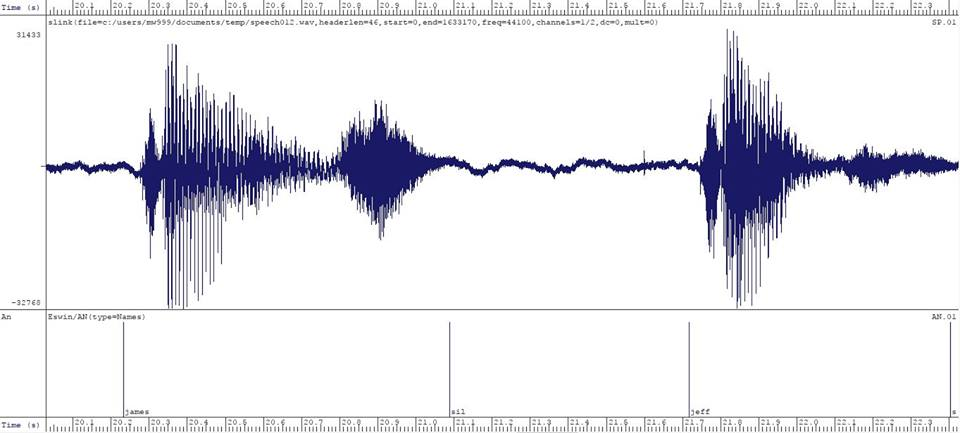
\includegraphics[width=60mm,scale=0.5]{sfs_example.jpg}\\
	\caption{Example of the SFS annotation process}\label{fig:sfs}
\end{figure}


\section{MFCC Feature Extraction}
Feature extraction, sometimes referred to as parameterisation or front-end processing, is an essential part in the development of a recogniser. The purpose of feature extraction is to take a time-domain representation of an audio signal, and extract information that can be used to classify the utterance. The information extracted is used for creating feature vectors. This is done because time-domain representations contain data that is not needed for the purpose of classification. This section outlines the feature extraction process used in the development of the recogniser.

\subsection{Block into frames}
The first step in feature extraction was to block the speech into frames. Speech articulators cannot move faster than 20ms, making the standard frame length 20ms \cite{framelength}. This equates to using a frame length of 320 samples when sampling at a rate of 16KHz, which is what was used in the audio recordings. Going forward, the feature extraction process is performed on these blocks individually, and then combined at the end to create a set of feature vectors for the entire utterance.

\subsection{Pre emphasis}
Pre emphasis was used to spectrally flatten the time-domain wave form. It does this by increasing the amplitude of high frequency bands, and decreasing that of the lower bands. In the recognisers implementation, a high-pass filter was used. It works by traversing the audio frame, sample-by-sample, and setting the value of each to be 97\% of the sample before it. Figure \ref{fig:preemphasis1} clearly shows the affect of pre emphasis. The turbulent waveform of the 'before' pre emphasis signal, shown in blue, is much smoother in the 'after' waveform, shown in magenta. This smoothing will make it easier and more consistent for the recogniser to classify utterances when training.

\begin{figure}[!htb]
	\centering
	\captionsetup{justification=centering}
	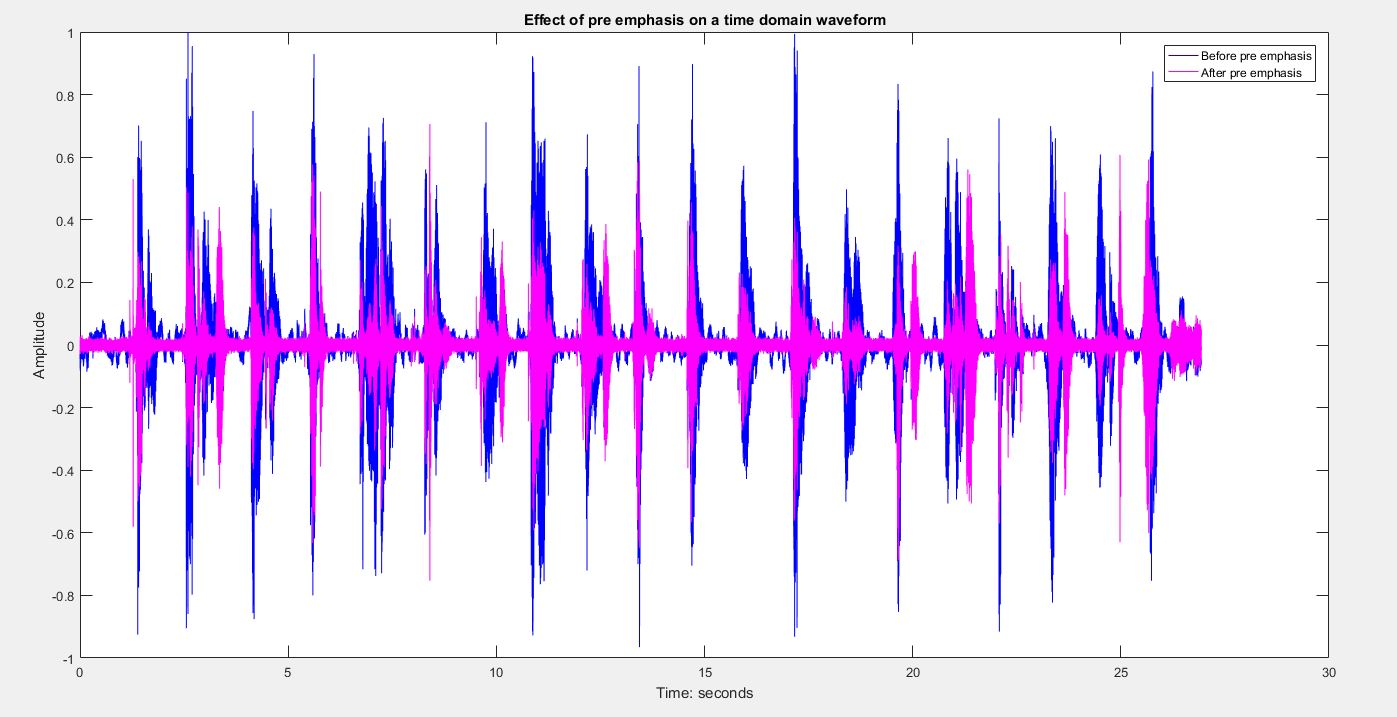
\includegraphics[width=0.5\textwidth]{pre_both.jpg}\\
	\caption{Effect of pre emphasis on a time domain waveform}\label{fig:preemphasis1}
\end{figure}

\subsection{Hamming window}
The next step was to apply a hamming window to the frame, which is also typically 20ms wide. Each hamming window is shaped as a bell curve, and overlaps half way with the hamming window either side of it. Figure \ref{fig:hamming} shows that as one window reaches its peak, the next is just starting, meeting in the middle.

\begin{figure}[!htb]
	\centering
	\captionsetup{justification=centering}
	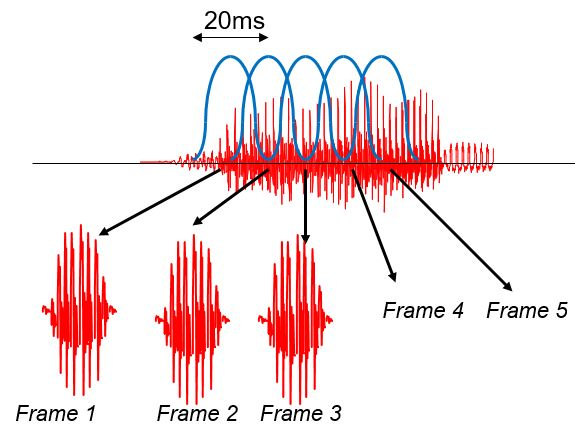
\includegraphics[width=0.4\textwidth]{hamming.jpg}\\
	\caption{Example of a hamming window applied to speech in the time-domain}\label{fig:hamming}
\end{figure}

The reason for applying the hamming window is that speech signals are non stationary, meaning over time they change rapidly. This rapid change makes any frequency analysis of the entire wave irrelevant. The wave therefore needs to be broken down into 20ms windows. It can be assumed that the characteristics of the speech will not change much over such a small period of time, which means they can be processed to gather their characteristics, and ultimately create the feature vectors. It is not a requirement for the windows to be bell shaped, or even overlapped at all, however these were found to give the best accuracy results for the recogniser.

\subsection{Spectral analysis}
A time-domain representation of a waveform can show how a speech signal changes over time. It can also be used to tell whether or not the speech is voiced or unvoiced. It does not provide much more than this however, which is why speech is typically analysed in the frequency domain. The frequency domain simply shows how many times an event occurred at each frequency during the entire period of observation. 

\begin{figure}[!htb]
	\centering
	\captionsetup{justification=centering}
	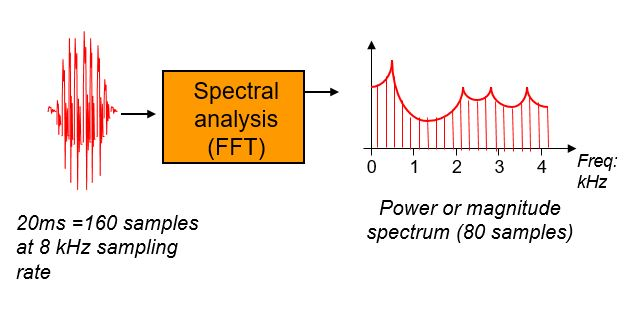
\includegraphics[width=0.4\textwidth]{specanal.jpg}\\
	\caption{Overview of the input and output of the spectral processing stage}\label{fig:specanal}
\end{figure}

When {\fontfamily{courier}\selectfont MATLAB's fft()} function is used in the recogniser, it produces a complex spectrum. This is because it contains information about the magnitude (real part), and phase (imaginary part), at each frequency. These can be extracted from the complex spectrum individually by using the {\fontfamily{courier}\selectfont abs()} and {\fontfamily{courier}\selectfont angle()} functions respectively on the spectrum.

Phase information is not useful in a recogniser as humans are not able to detect changes in phase when listening to audio. For this reason, the phase information at this phase in our feature extracting is discarded, favouring the magnitude information.

Figure \ref{fig:specanal} shows an overview of the spectral analysis process, displaying the number of samples going in, 160, is halved in the magnitude spectrum. This is because the magnitude spectrum is mirrored, as seen in figure \ref{fig:magspecexample}. This mirroring happens because as the number of samples increase when calculating the fourier transform, the phase of the cosine wave used for calculating the correlation changes. This also happens for the sine part used for calculating the phase. This will eventually result in the phase shift of 180 degrees at the last sample, thus giving an even reflection after half the samples. Because of this we cut off the reflected part of the data, halving the number of samples in the magnitude spectrum.

\begin{figure}[H]
	\centering
	\captionsetup{justification=centering}
	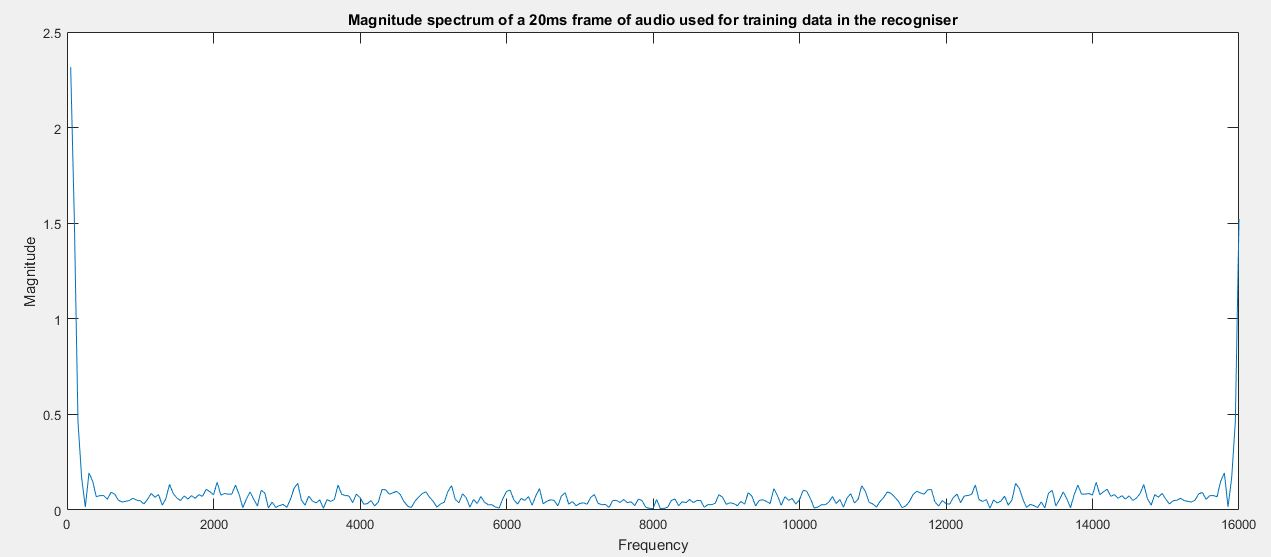
\includegraphics[width=0.4\textwidth]{magSpecExample.jpg}\\
	\caption{Result of plotting the magnitude spectrum taken from a 20ms frame of audio}\label{fig:magspecexample}
\end{figure}

\subsection{Filter Banks}
At this stage, the newly halved magnitude spectrum of the 20ms frame has been acquired. The next step is to take this and create a series of filter bank channels to represent the frame. In the recognisers implementation, a function was created to take in a magnitude spectrum as an argument, and return an MFCC vector. This recogniser implemented two types of filter banks: a {\fontfamily{courier}\selectfont mel-scale} implementation, and a {\fontfamily{courier}\selectfont linear} one.\\

\subsubsection{Linear}
A linear filter bank works by breaking the magnitude spectrum data points (samples) up into equal sections, taking the mean value of each section, and using this value to produce an {\fontfamily{courier}\selectfont MFCC}. The size of the sections, known as filterbank channels, can be adjusted in order to achieve greater accuracy of the system. Since there were 160 data points in the magnitude spectrum, the number of channels chosen in the initial implementation was 32, since it divides into 5 samples per channel.

The main benefit of the linear filter bank implementation is that it is much simpler. By implementing it first, the whole pipeline can be tested and any issues can be resolved. Once the pipeline is known to be in working order, a mel-scale filter bank can be implemented to improve the accuracy.

The drawbacks of the linear filter bank implementation is that it is not as accurate as the mel-scale. While it is possible to achieve good accuracy on a project with a small scope such as this one, it would not be sufficient for a project that seeks to recognise individual phonemes that are not in a pre-defined list. \\

\subsubsection{Mel-scale}
A mel-scale filter bank implementation seeks to mimic the way the human hearing works. The same concepts of breaking the data points (samples) up into sections and performing arithmetic on them is present, but with different methods of calculations. The shape of a mel-scale channel can be seen in figure \ref{fig:mel}.

\begin{figure}[!htb]
	\centering
	\captionsetup{justification=centering}
	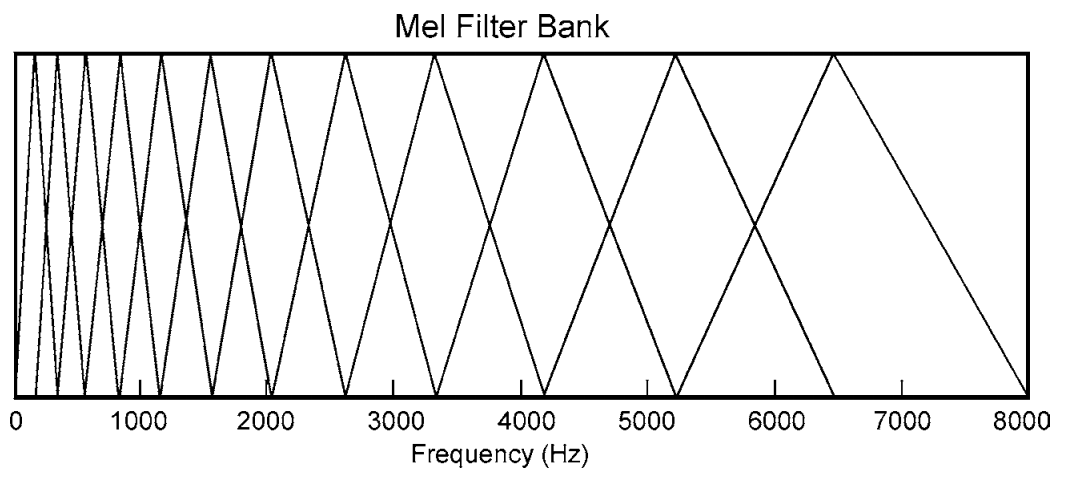
\includegraphics[width=0.4\textwidth]{mel.jpg}\\
	\caption{Mel-scale channels increasing in size as the frequency increases, from \cite{melpic}}\label{fig:mel}
\end{figure}

The first difference is the amount of samples in each channel. Instead of arbitrarily choosing a channel size to get the best accuracy, the sample size of each consecutive channel is increased using the mel-scale. The total number of channels is still a constant value. To fairly compare results of the first mel and linear implementations, 32 channels were used again.

As the channel size increased so does the frequency, this is because it mimics how humans hear sounds, using a logarithmic scale. Much more information can be extracted from lower frequency sounds so it makes sense for the channel sizes to be small, as to not obscure the important data. When the frequency is high however, we want to group the data points in a large channel, to ensure more emphasis is put into the lower frequency data when constructing the MFCCs.

The introduction of the mel-scale filterbank significantly improved the overall accuracy of the recogniser. The testing of this can be seen in section \ref{evaluation}.

\subsection{Log, DCT, and Truncation}
Assuming there are 32 channels, the output of the filter bank for each 20ms frame of speech is a vector containing 32 values. These are known as the filter bank energies. At this point, the log of the values is taken. The reason for this, as mentioned before, is that humans hear noise on a logarithmic scale. The consequence of this is that large variations in energy may not sound very different if the sound is loud to begin with \cite{melpic}. The affect the log has is to compress the channel values to match more closely what a human would hear. The MATLAB function used to achieve this was {\fontfamily{courier}\selectfont log10()}.

The next and final step to creating the MFCC is to DCT and truncate the now logged data vector. As shown in figure \ref{fig:mel}, the channels in the mel-scale filter bank are overlapped. This means that all the energies calculated and stored in the filter bank are closely correlated with each other. The goal is decorrelate them to allow the HMM classifier, covered in section \ref{AM}, to model the features properly. Once the DCT is applied, the values are truncated. This is because the result of the DCT will separate vocal tract information, stored in the lower-quefrency coefficients, from the excitation information, stored in the higher-quefrency coefficients. This excitation information is removed as it is useless in speech recognition, reducing the quality of the recogniser if present.


\section{Acoustic Modelling}\label{AM}
Hidden Markov Models (HMMs) were used as the classification algorithm for the recogniser, and has been one of the popular modelling techniques for over 20 years \cite{eddy1996hidden}. The recogniser went through a multitude of implementations, with the properties of the HMMS being adjusted each time to ensure the best accuracy. On a high level, each `state' of the model is meant to correspond to a stationary part of the signal, and from that a transition probability can be obtained to decide whether or not to move into the next state. So the feature vectors that were obtained earlier are each allocated to different HMM states, and this is used for training the recogniser. Once the recogniser has been trained using the feature data of the training utterances, it is ready to be tested. When testing, it will compare the test utterance data to the test data it previously computed, and return the most likely name using the calculated probabilities.

\begin{figure}[!htb]
	\centering
	\captionsetup{justification=centering}
	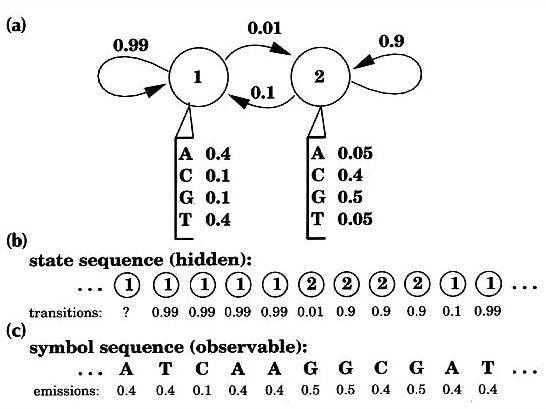
\includegraphics[width=0.4\textwidth]{hmm_example.jpg}\\
	\caption{Example of a Hidden Markov Model, from \cite{eddy1996hidden}}\label{fig:hmm}
\end{figure}

The HMM implementation was done using the HTK toolkit. The initial HMMs were calculated and then re-estimated using HRest, which improved the recognisers accuracy. It was found that 17 different HTK states produced the best accuracy, which will be discussed further in section \ref{evaluation}. 


\section{Noise Compensation}
Noise was added to the clean speech files to create noisy speech. This allowed the recogniser to be trained with sound that was more representative of a real world scenario. The noise added consisted of three files: background noise from a restaurant, noise from a factory, and the sound of a firing machine gun. All three types of noise were added to each of the ten training recordings, resulting in 30 new sound files. See Figure \ref{fig:noise} for an example of the difference in amplitude of a speech file with and without added noise.

\begin{figure}[!htb]
	\centering
	\captionsetup{justification=centering}
	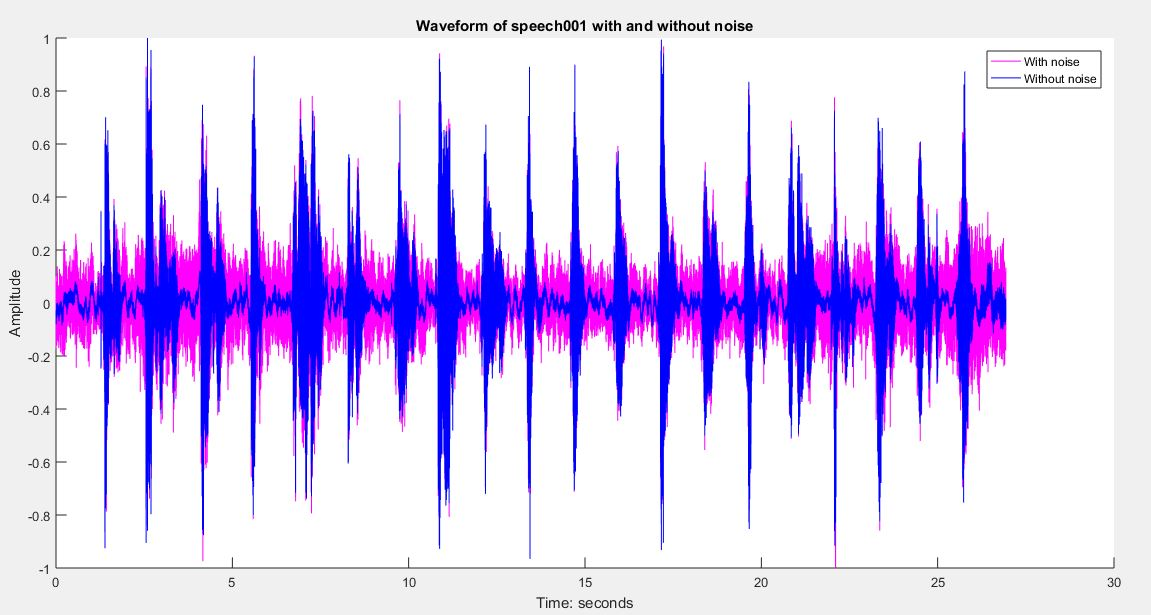
\includegraphics[width=0.5\textwidth]{noise_effect.jpg}\\
	\caption{Illustration of a speech file before and after noise was added}\label{fig:noise}
\end{figure}

Training the recogniser with the noisy speech resulting in a lower accuracy percentage as expected when testing with noise free data. The accuracy increased when tested with noisy speech data, but not by much. This will be covered further in section \ref{evaluation}.


\section{Evaluation}\label{evaluation}
	This section will outline the results of the implementation testing through the life cycle of the speech recogniser. The highest accuracy achieved by the recogniser was \textbf{97.78\%}. The characteristics of the recogniser used to achieve this result were:
	
	\begin{enumerate}
		\item Pre emphasis applied
		\item 20ms audio frames with a 50\% overlap
		\item 32 channel mel-scale filterbank
		\item Post DCT truncation of half the data points
		\item 16 state HMM model in HTK
		\item HRest used to re-estimate the HMMs
	\end{enumerate}

	Since the accuracy was so high at this point, it was not easy to see the individual impact when changing any of these characteristics. To this end, noise was added to the speech training files to bring the overall accuracy of the system down. This allowed for better analysis of each characteristic. Applying factory noise to the training files provided an overall accuracy of \textbf{74.26\%}. Knowing this accuracy allowed us to modify the individual components inside the feature extraction process and see what the resulting accuracy was. Going forward it is important to note that only one characteristic was changed at a time.
	
	\subsection{Pre Emphasis}
	The first test performed was testing the accuracy discrepancy when the pre emphasis is removed from the feature extraction process. The results can be seen in figure \ref{fig:eval_pre}.
	\\
	\begin{figure}[!htb]
		\centering
		\captionsetup{justification=centering}
		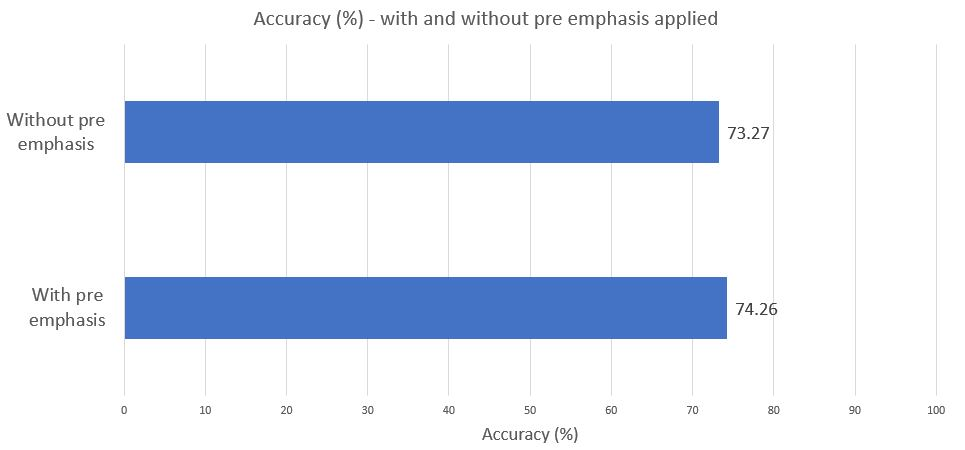
\includegraphics[width=0.5\textwidth]{eval_pre.jpg}\\
		\caption{Effect of pre emphasis on accuracy when using a noisy signal. }\label{fig:eval_pre}
	\end{figure}
	
	Pre emphasis improved the accuracy, but not by very much. The reason for this is likely due to the amount of noise present in the audio signal. When the signal waveform is relatively noise free, pre emphasis can smooth the signal and reduce the impact of noise very well. However when the waveform is very noisy, the noise impact can be reduced, but to a lesser extent. This theory is supported by figure \ref{fig:eval_pre_nonoise} which shows a greater increase in accuracy when pre emphasis is applied to the relatively noise free signal used for training and testing the recogniser.
	\\
	\begin{figure}[!htb]
		\centering
		\captionsetup{justification=centering}
		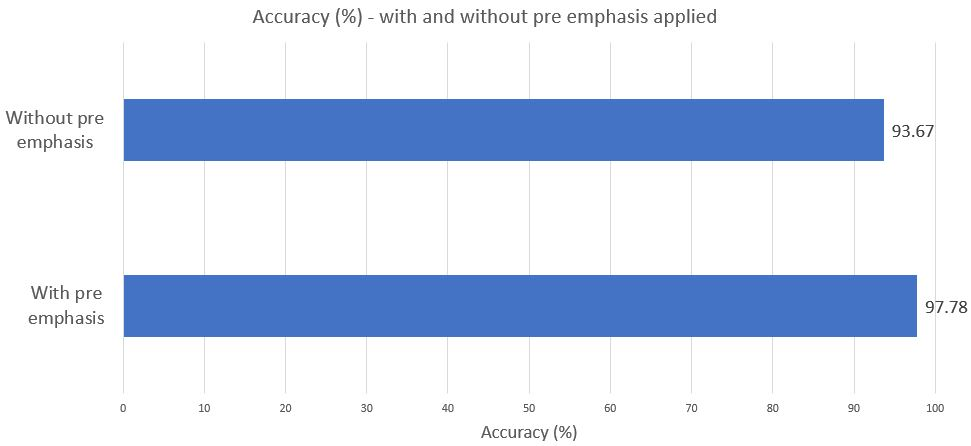
\includegraphics[width=0.5\textwidth]{eval_pre_nonoise.jpg}\\
		\caption{Effect of pre emphasis on accuracy when using a relatively noise free signal. }\label{fig:eval_pre_nonoise}
	\end{figure}

	\subsection{Filterbanks}
	As mentioned in the evaluation introduction, a 32 channel mel-scale filter bank was used in the best accuracy implementation of the recogniser. The affect of different numbers of channels is an interesting idea that was explored. Figure \ref{fig:eval_filterbanks} shows the results of the tests. It is important to note that after acquiring the filter bank values, the log and DCT stages were applied, and half the result truncated to remain consistent with the initial evaluation accuracy.
	\\
	
	\begin{figure}[!htb]
		\centering
		\captionsetup{justification=centering}
		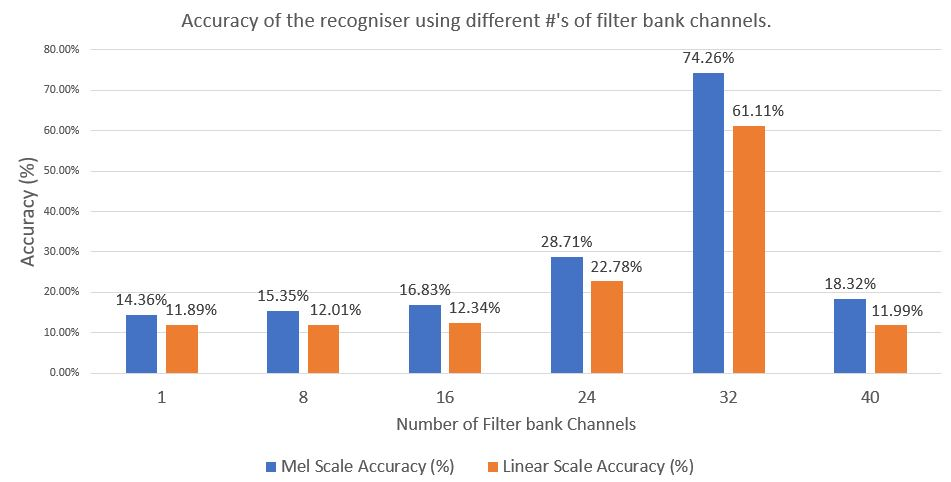
\includegraphics[width=0.5\textwidth]{eval_filterbanks.jpg}\\
		\caption{Accuracy (\%) of the recogniser when using different numbers of filter bank channels}\label{fig:eval_filterbanks}
	\end{figure}

	The recogniser was implemented with both linear (shown in orange) and a mel (shown in blue) scale filter bank channels. The mel scale implementation provided better accuracy at every stage of testing, which is expected due to the way in which it calculates channel size. A channel size of 32 provided the best accuracy in both filter bank implementations. This is because it means there are enough channels to represent the data without obscuring it too much. Too many channels will result in the high frequency data, which is not useful for audio speech recognition, having a larger impact on the training process which decreases the accuracy.
	
	Since there was such a large spike in accuracy after 24 channels, which quickly goes back down at 40 channels, some further analysis was performed - looking at the channels in between these two. The results can be seen in figure \ref{fig:eval_filterbanks_zoom}. It shows that the accuracy does increase gradually, instead of just spiking dramatically. The accuracy does increase and decrease very quickly after peaking at 32 channels.
	
	\begin{figure}[!htb]
		\centering
		\captionsetup{justification=centering}
		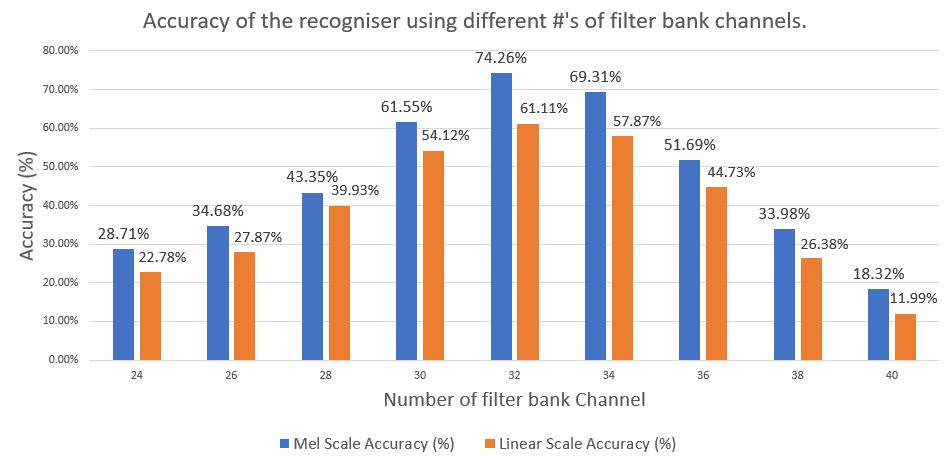
\includegraphics[width=0.5\textwidth]{eval_filterbanks_zoom.jpg}\\
		\caption{Accuracy (\%) of the recogniser when using different numbers of filter bank channels}\label{fig:eval_filterbanks_zoom}
	\end{figure}
	
	Although the best overall accuracy of the recogniser was 97.78\% using a mel scale filter bank, we were able to achieve slightly less than this (~96\%) using a linear filter bank. This is probably due to the fact that the data set used for acquiring these results is just 20 words, which is a relatively simple procedure. If the complexity of the system is increased, then the differences in accuracy would be further highlighted.
	
	\subsection{Truncation}
	Assuming that 32 filter bank channels are being used, the next test was to decide how much data should be truncated to improve accuracy. As mentioned in section \ref{ldt}, the purpose of truncation in this recogniser implementation is to eliminate the excitation data from the signal before writing the HTK files. To see the affect of changing the level of truncation, measures were taken at:
	\begin{itemize}
		\item Samples 1 to 32 kept (no data deleted)
		\item Samples 1 to 24 kept (25\% of data deleted)
		\item Samples 1 to 16 kept (50\% of data deleted)
		\item Samples 1 to 8 kept (75\% of data deleted)
		\item Sample 1 kept only (96.875\% data deleted)
	\end{itemize}

	\begin{figure}[H]
		\centering
		\captionsetup{justification=centering}
		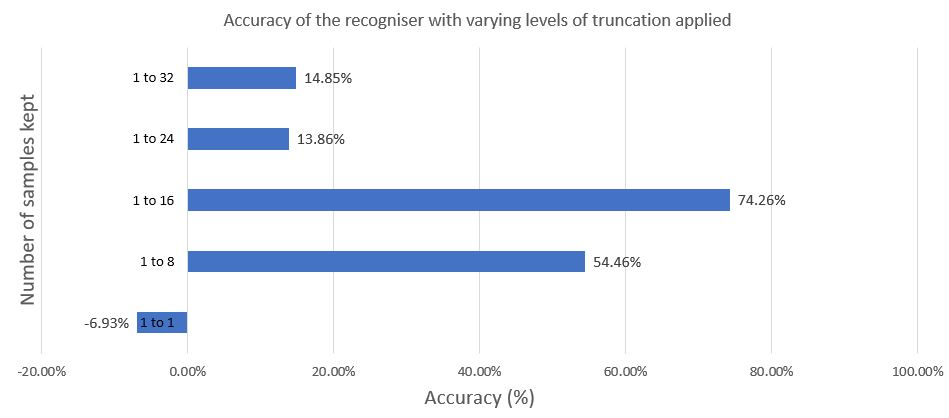
\includegraphics[width=0.5\textwidth]{eval_truncation.jpg}\\
		\caption{Accuracy (\%) of the recogniser when using different levels of truncation}\label{fig:eval_truncation}
	\end{figure}

	Figure \ref{fig:eval_truncation} shows that the most effective level of truncation is around 50\%. As discussed before, this is generally the industry standard for speech recognisers. The difference between keeping samples 1-16 and samples 1-24 is much lager than the difference between keeping 1-16 and 1-8. This is because the acoustic information is stored in the early samples; so if 24 samples are kept, too much excitation data gets through, which reduces the accuracy significantly. Keeping just one sample provided a negative accuracy, which is expected since every sample will be considered when calculating the output.
	
	\subsection{HMM States}
	The number of HMM states also had a large impact on the overall accuracy of the recogniser. To test this impact, an HMM model was created for states ranging from 1 to 20, and each was used on the same training data to achieve an accuracy measurement. The results of these tests can be seen in figure \ref{fig:eval_hmm}. States lower than 6 were purposefully omitted from the graph to avoid diluting the values of the axis as the resulting accuracy was trivially small, reaching an accuracy of below -1000\%.

	\begin{figure}[H]
		\centering
		\captionsetup{justification=centering}
		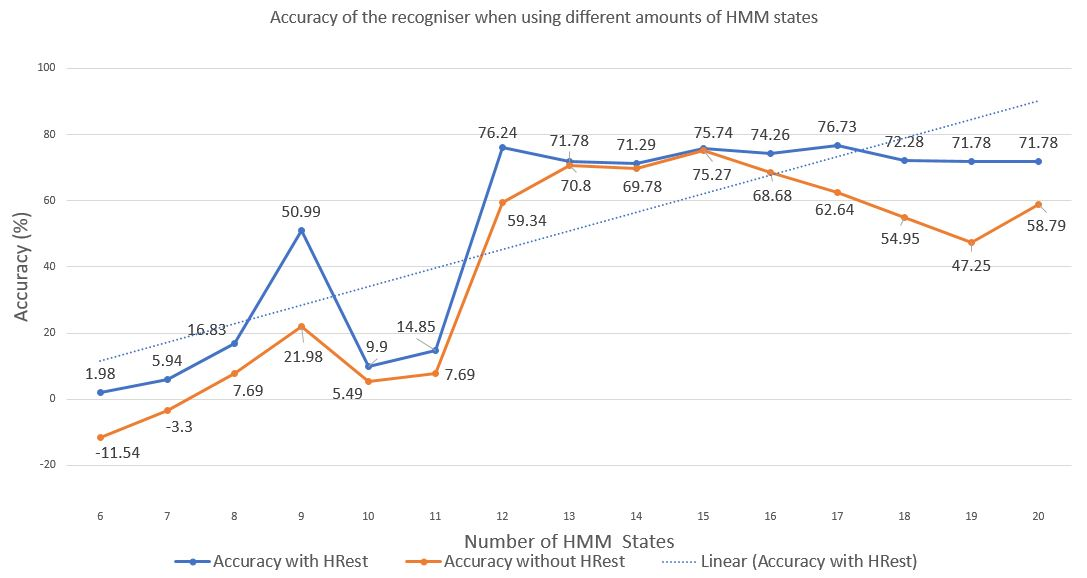
\includegraphics[width=0.5\textwidth]{eval_hmm.jpg}\\
		\caption{Accuracy (\%) of the recogniser when using different \#'s of HMM states}\label{fig:eval_hmm}
	\end{figure}

	
	
	One of the most interesting features of these results is the large spike in accuracy at 9 states. It seems unintuitive for such a spike to occur for 9 states, and then drop down so significantly for 10 states - however the pipeline was thoroughly inspected and no problems were found. 
	
	A possible cause of this spike is that the names in spoken for the purpose of training and testing this recogniser break down well into ~9 different states, which would also explain why the recogniser reaches its peak in accuracy when using roughly double (17) the states. As mentioned in section \ref{AM}, each state will ideally correspond to one `stationary' part of the signal.
	
	Also interestingly, it was found during the testing for this stage that a 17 state HMM model provided greater accuracy than the 16 state model which was initially assumed to be the peak accuracy of this recogniser.

	\subsection{HRest vs HInit}
	HRest is part of the HTK toolkit that is used to re-estimate the initial HMMs to improve the accuracy of the recogniser. The original HMMs are obtained using HInit, which uses the Viterbi algorithm to calculate the probability of moving to the next state in the model, which is defined using characteristics of the MFCCs obtained during feature extraction. The number of states used in the recogniser was 16.
	
	HRest uses the output from HInit directly to create it's re-estimated result. It uses the Baum-Welch algorithm to do this. The results of HRest are significant, as can be seen by the orange line in figure \ref{fig:eval_hmm}. The accuracy at every state using HInit alone is lower than its respective implementation with HRest applied. The results do tend to follow the same trend line however.

\section{Conclusions}
This report presented several different methods for implementing a speech recogniser. There are many different parameters used during the feature extraction process that can be tweaked to provide drastically different results. Some aspects of the process are set in stone however, such as pre-emphasis, which is always better to include than omit. 

The results from the methods used to transform frequency to MFCCs were found to be universally better when using a mel-scale filterbank, since it's methods for determining channel size are designed to mimic the way we hear. The other characteristics of the feature extraction process, like truncation and the number of channels, all seemed to show that there is definitely a `best way' of doing things in this process.

\bibliographystyle{apalike}
\bibliography{avp_bib} 
\end{document}